%----------------------------------------------------------------------------
\chapter{\kubernetes}
%----------------------------------------------------------------------------
\section{Kubernetes bemutatása}
Láthattuk, hogy ahogy nő a rendszerben a telepíthető alkalmazáskomponensek száma, egyre nehezebb lesz mindegyiket kezelni.
A Google volt valószínűleg az első vállalat, amely felismerte, hogy sokkal jobb módszerre van szüksége a szoftverkomponensek telepítéséhez és kezeléséhez, valamint a globálisan skálázható infrastruktúrájához.
Egyike annak a kevés vállalatnak a világon, amely több százezer szervert üzemeltet, és amelynek a telepítések kezelésével kell foglalkoznia ilyen hatalmas léptékben.
Ez arra kényszerítette őket, hogy olyan megoldásokat dolgozzanak ki, amelyekkel több ezer szoftverkomponens fejlesztése és telepítése kezelhetővé és költséghatékonnyá tehető.

A Kubernetes egy olyan szoftverrendszer, amely lehetővé teszi, hogy egyszerűen telepítsünk és kezeljünk rajta konténeres alkalmazásokat.
A Linux konténerek funkcióira támaszkodik, hogy heterogén alkalmazásokat futtasson anélkül, hogy ismernie kellene ezen alkalmazások belső részleteit, és anélkül, hogy ezeket az alkalmazásokat manuálisan kellene telepíteni az egyes hosztokon.
Mivel ezek az alkalmazások konténerekben futnak, nem befolyásolják az ugyanazon a szerveren futó többi alkalmazást, ami kritikus fontosságú, ha teljesen különböző szervezetek alkalmazásait futtatja ugyanazon a hardveren.
Ez a felhőszolgáltatók számára kiemelkedő fontosságú, mivel a hardverük lehető legjobb kihasználására törekszenek, miközben a hosztolt alkalmazások teljes elszigeteltségét is fenn kell tartaniuk.
A Kubernetes lehetővé teszi, hogy szoftveralkalmazásait több ezer számítógépcsomóponton futtassa, mintha ezek a csomópontok mind egyetlen, hatalmas számítógép lenne.
Absztrahálja a mögöttes infrastruktúrát, és ezáltal egyszerűsíti a fejlesztést, a telepítést és a kezelést mind a fejlesztő, mind az üzemeltetési csapatok számára.
Az alkalmazások telepítése a Kubernetes segítségével mindig ugyanaz, függetlenül attól, hogy a klaszter (későbbiekben cluster) csak néhány csomópontot (későbbiekben node) tartalmaz vagy több ezret.
A cluster mérete egyáltalán nem számít.
A további node-ok egyszerűen a telepített alkalmazások számára rendelkezésre álló erőforrások további mennyiségét jelentik \cite{Marko17}.

\section{A Kubernetes működésének megértése}
A rendszer egy fő csomópontból (későbbiekben master node) és tetszőleges számú munkás csomópontból (későbbiekben worker node) áll.
Amikor a fejlesztő elküldi az alkalmazások listáját a master-nek, a Kubernetes telepíti azokat a worker node-okra (lásd \ref{kubernetes-overview} ábrán).
Az, hogy egy komponens melyik worker node-on landol, nem számít (és nem is szabadna számítania) sem a fejlesztőnek, sem a rendszergazdának.
A fejlesztő megadhatja, hogy bizonyos alkalmazásoknak együtt kell futniuk, és a Kubernetes ugyanarra a worker node-ra telepíti őket.
Mások szétszóródnak a cluster-ben, de ugyanúgy tudnak egymással kommunikálni, függetlenül attól, hogy hova telepítik őket \cite{Marko17}.

\begin{figure}[ht]
    \centering
         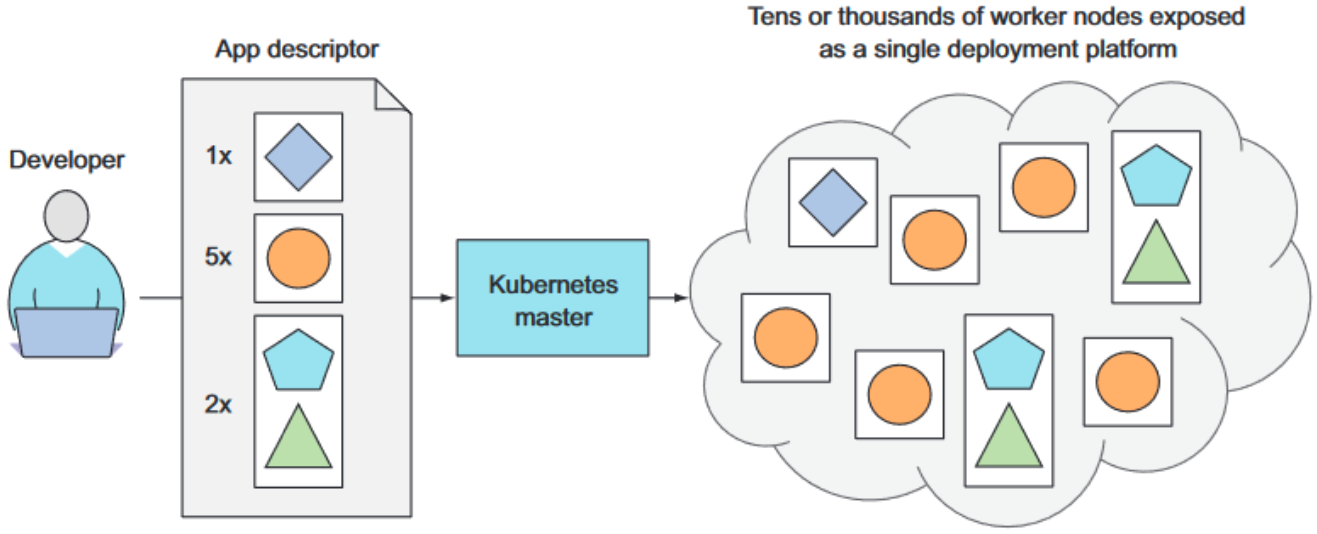
\includegraphics[width=1.0\textwidth]{figures/kubernetes/kubernetes-overview.png}
          \caption{A Kubernetes, mint egyetlen telepítési platform \cite{Marko17}.}
           \label{kubernetes-overview}
\end{figure}

Hardveres szinten egy Kubernetes cluster sok node-ból áll, amelyek két típusra oszthatók:
\begin{itemize}
    \item A master node, amely a Kubernetes vezérlőjének (későbbiekben Control Plane) ad otthont, amely az egész Kubernetes rendszert irányítja és kezeli.
    \item A worker node, amely a tényleges telepített alkalmazásokat futtatja.
\end{itemize}

\newpage

\subsection{A Control Plane}
A Control Plane az, ami a cluster-t irányítja és működésre készteti.
Több komponensből áll, amelyek egyetlen master node-on futhatnak, vagy több node-ra oszthatók és replikálhatók a magas rendelkezésre állás biztosítása érdekében.
Ezek az összetevők a következők:
\begin{itemize}
    \item Az API szerver, amellyel a felhasználó és a többi control plane komponens kommunikál.
    \item Az ütemező (későbbiekben Scheduler), amely ütemezi az alkalmazásokat (az alkalmazás minden telepíthető komponenséhez hozzárendel egy worker node-ot).
    \item A vezérlő menedzser (későbbiekben Controller Manager), amely cluster szintű funkciókat lát el, mint például a komponensek replikálása, a munkás node-ok nyomon követése, a node-ok hibáinak kezelése stb.
    \item etcd, egy megbízható elosztott adattároló, amely tartósan tárolja a cluster konfigurációját.
\end{itemize}
A Control Plane összetevői tartják és vezérlik a cluster állapotát, de nem futtatják az alkalmazásokat (lásd \ref{cluster-overview} ábrán). Ezt a worker node-ok végzik \cite{Marko17}.

\subsection{A worker node-ok}
A worker node-ok azok a gépek, amelyek a konténerizált alkalmazásokat futtatják (lásd \ref{cluster-overview} ábrán).
Az alkalmazások futtatásának, felügyeletének és szolgáltatásnyújtásának feladatát a következő komponensek végzik: \cite{Marko17}
\begin{itemize}
    \item Docker, rkt vagy más konténer futtató, amely futtatja a konténereket.
    \item A Kubelet kommunikál az API-kiszolgálóval és kezeli a konténereket a node-ján.
    \item A Kubernetes Service Proxy (kube-proxy), amely elosztja a hálózati forgalmat az alkalmazáskomponensek között.
\end{itemize}

\begin{figure}[ht]
    \centering
         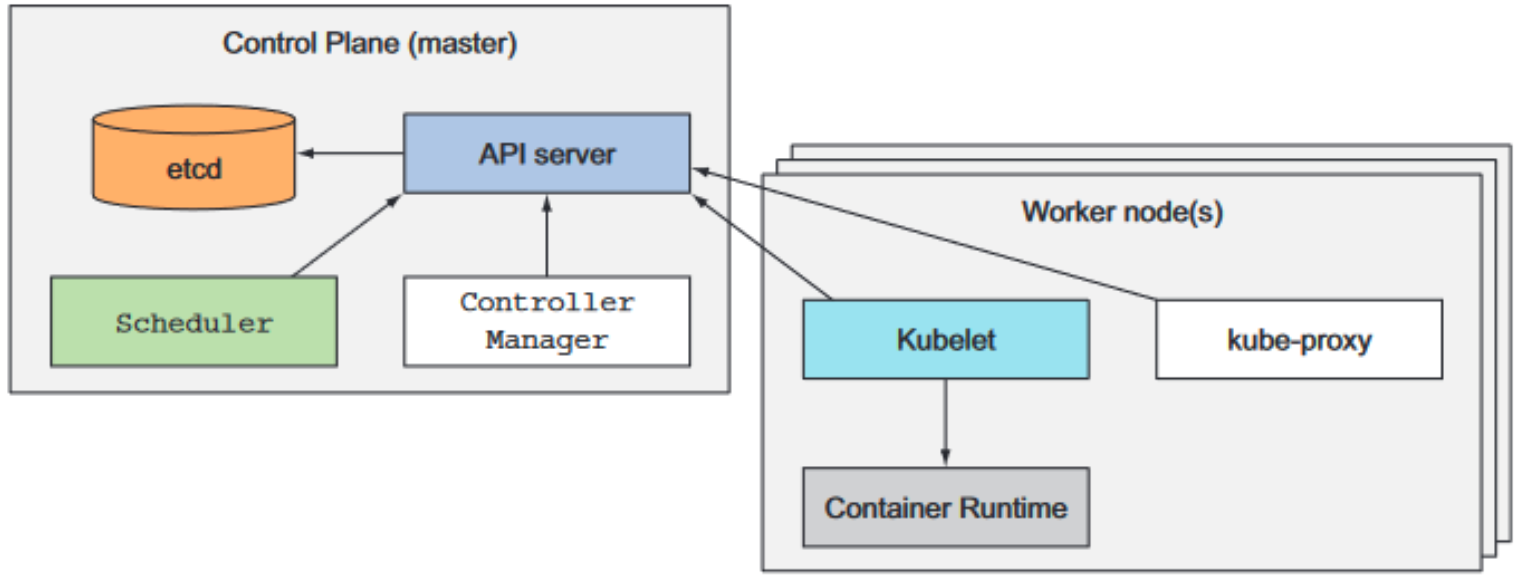
\includegraphics[width=1.0\textwidth]{figures/kubernetes/cluster-overview.png}
          \caption{A Kubernetes cluster-t alkotó komponensek \cite{Marko17}.}
           \label{cluster-overview}
\end{figure}

\subsection{A podok bevezetése}
A Kubernetes nem foglalkozik közvetlenül az egyes konténerekkel.
Ehelyett a több, együtt elhelyezett konténer koncepcióját használja.
Ezt a konténerekből álló csoportot podnak nevezzük.
A pod egy vagy több szorosan összefüggő konténer csoportja, amelyek mindig ugyanazon a worker node-on és ugyanazon a linux névtereken futnak együtt.
Minden pod olyan, mint egy különálló logikai gép, saját IP-vel, hostnévvel, folyamatokkal, amely egyetlen alkalmazást futtat (lásd \ref{node-pod-scheduler} ábrán).
Az alkalmazás lehet egyetlen folyamat, amely egyetlen konténerben fut, vagy lehet egy fő alkalmazási folyamat és további támogató folyamatok, amelyek mindegyike saját konténerben fut.
Egy podban lévő összes konténer látszólag ugyanazon a logikai gépen fut, míg a többi podban lévő konténerek, még ha ugyanazon a worker node-on futnak is, látszólag másikon futnak \cite{Marko17}.

\begin{figure}[ht]
    \centering
         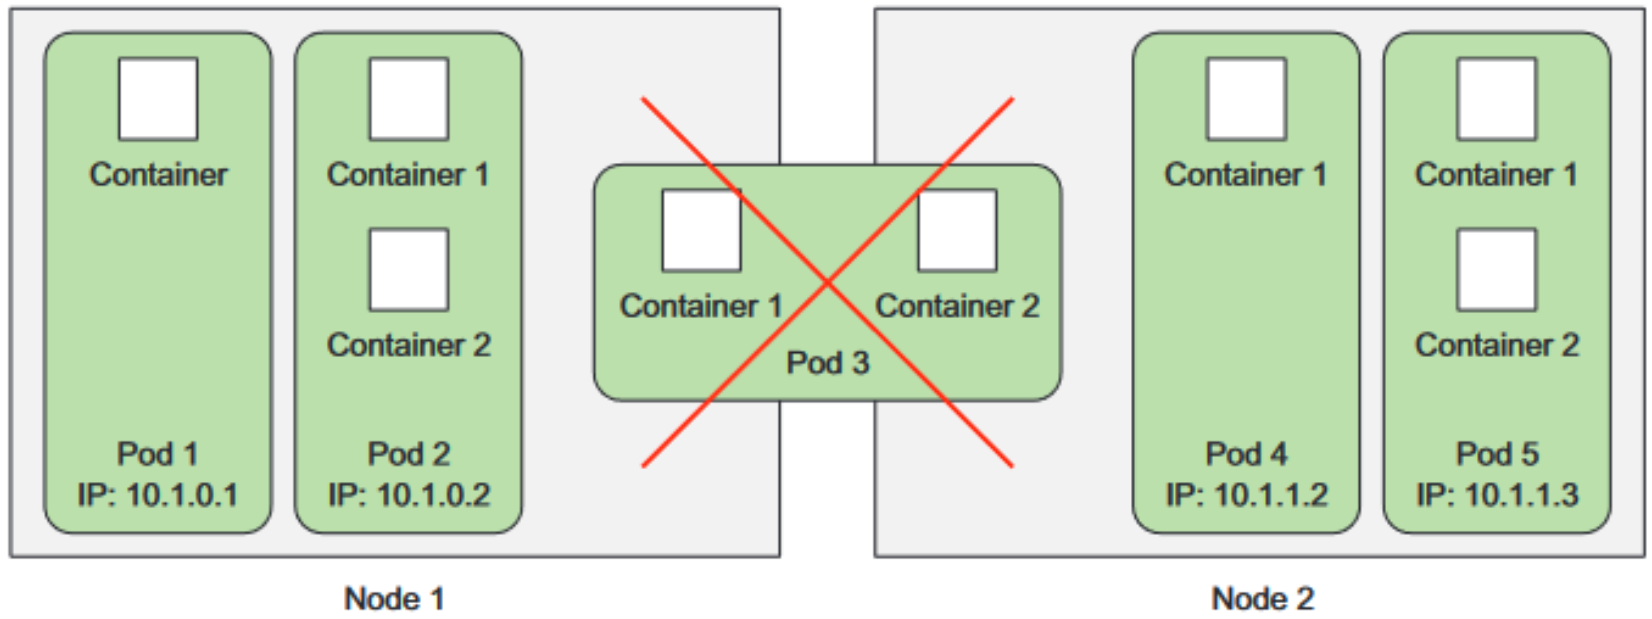
\includegraphics[width=1.0\textwidth]{figures/kubernetes/node-pod-scheduler.png}
          \caption{Egy pod minden konténere ugyanazon a node-on fut. Egy pod soha nem terjed ki két node-ra \cite{Marko17}.}
           \label{node-pod-scheduler}
\end{figure}

\subsection{A Service bemutatása}
A Kubernetes Service egy olyan erőforrás, amelyet azért hozunk létre, hogy egyetlen, állandó belépési pont legyen egy podok csoportjához, amelyek ugyanazt a szolgáltatást nyújtják.
Minden szolgáltatásnak van egy IP-címe és portja, amelyek a szolgáltatás létezése alatt soha nem változik.
Az felhasználók kapcsolatot nyithatnak az adott IP-címre és portra és ezek a kapcsolatok az adott szolgáltatást támogató podok egyikéhez kerülnek továbbításra.
Így a szolgáltatás felhasználóinak nem kell ismerniük a szolgáltatást nyújtó egyes podok helyét és címét, így ezek a podok bármikor áthelyezhetők a cluter-en belül (lásd \ref{service-overview} ábrán) \cite{Marko17}.

\begin{figure}[ht]
    \centering
         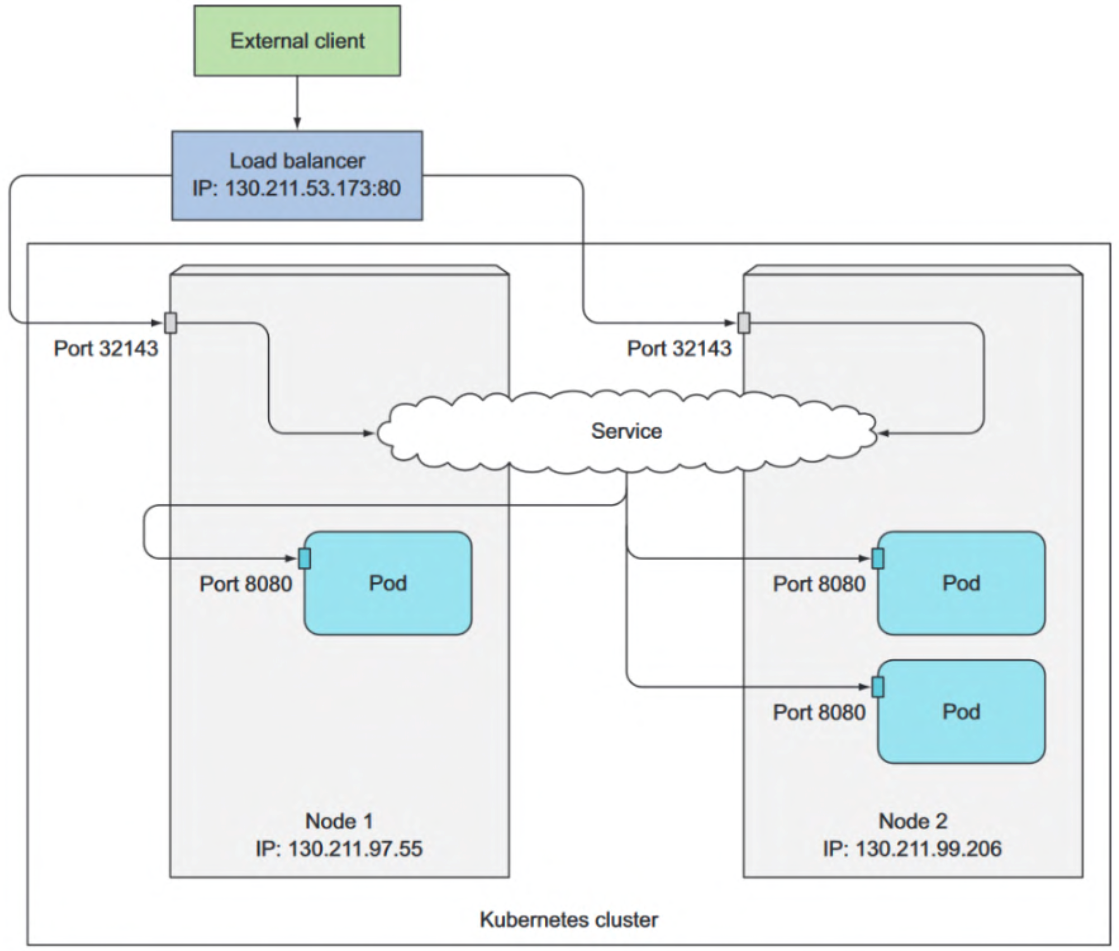
\includegraphics[width=0.9\textwidth]{figures/kubernetes/service-overview.png}
          \caption{Szolgáltatás megnyitása külső felhasználók számára \cite{Marko17}.}
           \label{service-overview}
\end{figure}

\subsection{A Secrets bemutatása}
A konfiguráció általában érzékeny információkat is tartalmaz, például hitelesítő adatokat és privát titkosítási kulcsokat, amelyeket biztonságban kell tartani.
Az ilyen információk tárolására és terjesztésére a Kubernetes egy különálló objektumot biztosít, amelyet Secretnek hívnak.
A titkok hasonlóak a ConfigMaps-hoz, ők is leképezések, amelyek kulcs-érték párokat tartalmaznak.
A Kubernetes segít megőrizni a Secrets biztonságát azzal, hogy minden Secret csak azokhoz a node-okhoz jut el, amelyek a Secret hozzáférésre szoruló podokat futtatják.
Emellett a node-okon maguk a Secret-ek mindig a memóriában tárolódnak, és soha nem íródnak fizikai tárolókra, ami a lemezek törlését igényelné a Secret törlése után. Magán a master node-on (pontosabban az etcd-ben) a Secret-eket korábban titkosítatlan formában tárolták, ami azt jelentette, hogy a master node-ot védeni kell az tárolt érzékeny adatok biztonsága érdekében.
Ez nem csak az etcd tárolás biztonságban tartására terjedt ki, hanem arra is, hogy megakadályozzuk, hogy illetéktelen felhasználók használhassák az API-kiszolgálót, mivel bárki, aki podokat tud létrehozni, fel tudja csatolni a secret-et a podba, és azon keresztül hozzáférhet az érzékeny adatokhoz.
A Kubernetes 1.7-es verziójától az etcd titkosított formában tárolja a Secret-eket, ami sokkal biztonságosabbá teszi a rendszert \cite{Marko17}.

\subsection{Kliens könyvtárak az API-kiszolgálóval való kommunikációhoz}
A Kubernetes közösségnek számos speciális érdekcsoportja és munkacsoportja van, amelyek a Kubernetes ökoszisztéma egyes részeire összpontosítanak.
Jelenleg két Kubernetes API klienskönyvtár létezik, amelyeket az API Machinery speciális érdekcsoport (SIG) támogat: \cite{Marko17}

\begin{itemize}
    \item Golang client (https://github.com/kubernetes/client-go)
    \item Python (https://github.com/kubernetes-incubator/client-python)
\end{itemize}

\subsection{Egyéni API-objektumok definiálása}
Ahogy a Kubernetes ökoszisztéma fejlődik, egyre több és több magas szintű objektumot fog látni, amelyek sokkal speciálisabbak lesznek, mint a Kubernetes által ma támogatott erőforrások.
Ahelyett, hogy Deployments, Services, ConfigMaps és hasonlókkal foglalkozna, egész alkalmazásokat vagy szoftverszolgáltatásokat reprezentáló objektumokat fog létrehozni és kezelni.

Egy egyéni vezérlő fogja megfigyelni ezeket a magas szintű objektumokat, és ezek alapján alacsony szintű objektumokat hoz létre.
Például ahhoz, hogy a webhelyobjektumok egy szolgáltatáson keresztül elérhető webkiszolgáló podot futtassanak, létre kell hoznia és telepítenie kell egy webhelyvezérlőt, amely figyeli az API-kiszolgálót a webhelyobjektumok létrehozására, majd létrehozza a szolgáltatást és a webkiszolgáló podot mindegyikhez (lásd \ref{custom-controller} ábrán).
Annak érdekében, hogy a Pod kezelt legyen és túlélje a node-ok hibáit, a vezérlő közvetlenül egy deployment erőforrást hoz létre a nem kezelt pod helyett \cite{Marko17}.

\begin{figure}[ht]
    \centering
         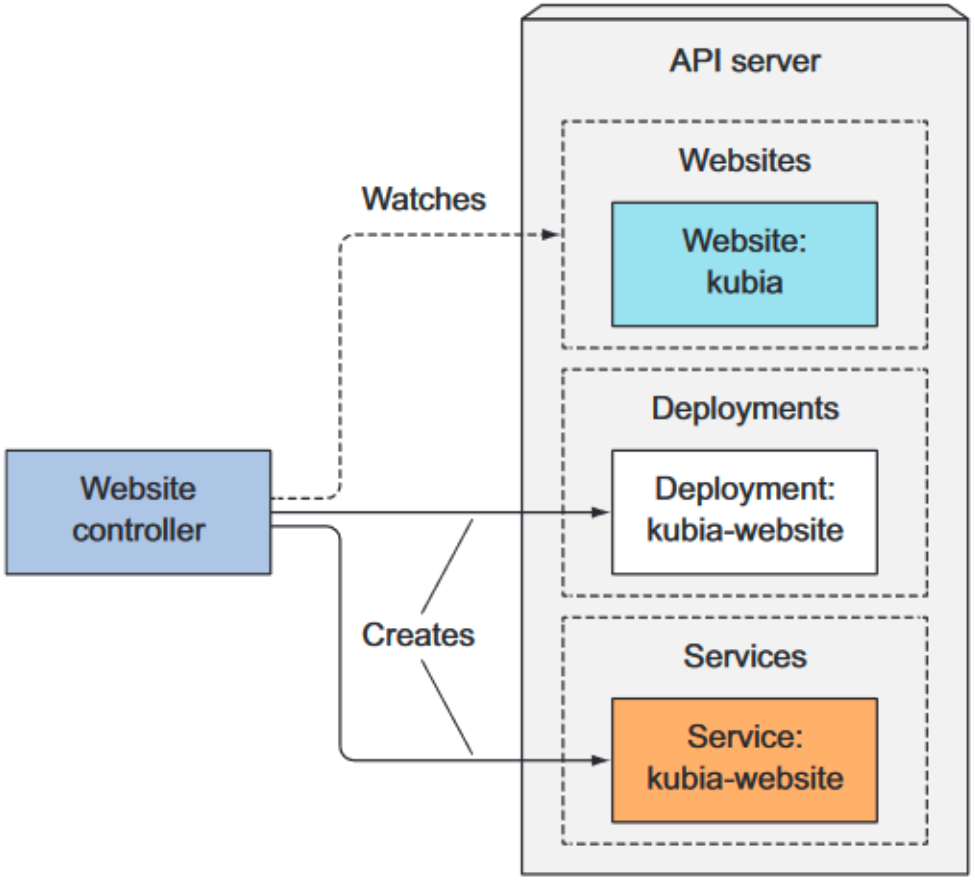
\includegraphics[width=0.85\textwidth]{figures/kubernetes/custom-controller.png}
          \caption{A weboldal controllere figyeli a webhely objektumokat és létrehoz egy deployment-et és egy service-t \cite{Marko17}.}
           \label{custom-controller}
\end{figure}

\newpage

\subsection{Az operátor bemutatása}
Az operátor egy Kubernetes-alkalmazás csomagolására, telepítésére és kezelésére szolgáló módszer. Egy Kubernetes-alkalmazást egyszerre telepítünk a Kubernetesre és kezelünk a Kubernetes API (alkalmazásprogramozási felület) és a kubectl tool (segédeszköz) segítségével.

A Kubernetes-operátor egy alkalmazásspecifikus vezérlő, amely a Kubernetes API funkcionalitását kiterjeszti, hogy komplex alkalmazások példányait hozza létre, konfigurálja és kezelje a Kubernetes-felhasználó nevében.
A Kubernetes erőforrás és vezérlő alapkoncepcióira épül, de magában foglalja a tartomány- vagy alkalmazásspecifikus tudást az általa kezelt szoftver teljes életciklusának automatizálása érdekében. 

A Kubernetesben a control plane vezérlői olyan vezérlési feladatokat valósítanak meg, amelyek ismételten összehasonlítják a cluster kívánt állapotát annak tényleges állapotával.
Ha a cluster tényleges állapota nem egyezik a kívánt állapottal, akkor a vezérlő lépéseket tesz a probléma kijavítására. 

Az operátor egy olyan egyéni Kubernetes vezérlő, amely egyéni erőforrást (későbbiekben custom resource vagy CR) használ az alkalmazások és komponenseik kezelésére.
A magas szintű konfigurációt és beállításokat a felhasználó adja meg egy custom resource-on belül.
A Kubernetes operátor a magas szintű utasításokat az operátor logikájába ágyazott legjobb gyakorlatok alapján fordítja le az alacsony szintű műveletekre.

A custom resource Kubernetes API-bővítési mechanizmusa.
Egy egyéni erőforrás-definíció (későbbiekben custom resource definition vagy CRD) definiál egy CR-t, és felsorolja az operátor felhasználói számára elérhető összes konfigurációt.
A Kubernetes-operátor figyeli a CR típusát, és alkalmazásspecifikus műveleteket hajt végre annak érdekében, hogy az aktuális állapot megfeleljen az erőforrás által kívánt állapotának.

A Kubernetes-operátorok új objektumtípusokat vezetnek be az CRD-k révén.
A CRD-t a Kubernetes API ugyanúgy kezelheti, mint a beépített objektumokat, beleértve a kubectl-en keresztüli interakciót és a szerepkör-alapú hozzáférés-szabályozásba (RBAC) való felvételt.
Az operátor továbbra is figyelemmel kíséri az alkalmazását, miközben az fut, és automatikusan biztonsági mentést készíthet az adatokról, helyreállíthatja a hibákat, és frissítheti az alkalmazást. 

A Kubernetes-operátor által végzett műveletek szinte bármi lehet: egy összetett alkalmazás skálázása, az alkalmazás verziófrissítése, vagy akár egy speciális hardverrel rendelkező számítási cluster node-jainak kernelmoduljainak kezelése \cite{RedHatKubOp}.

Az Istio operátor felépítése látható \ref{operator-overview} ábrán.

\newpage

\section{Kubernetes in Docker}
A Kubernetes in Docker (későbbiekben kind) egy eszközcsomag a helyi Kubernetes cluster-ekhez, ahol minden node egy Docker konténer. A kind a Kubernetes tesztelését célozza meg.

A kind funkcionalitásának nagy részét megvalósító go csomagokra, a felhasználóknak szánt parancssorra és egy node base image-re (alap lemezképre) oszlik. A szándék az, hogy a kind csomagjai importálható és újrafelhasználható legyen más eszközök (pl. kubetest) által, míg a CLI gyors módot biztosít e csomagok használatára és hibakeresésére.

Bár nem minden tesztelés végezhető el valódi cluster-ek nélkül a felhőben, de elég lehet ahhoz, hogy ha valami ilyesmit akarunk: \cite{KinD}
\begin{itemize}
    \item Nagyon olcsó cluster-eket futtatni, amelyeket bármely fejlesztői környezetben replikálhatóak.
    \item Integrálható más eszközökkel.
    \item Aslaposan dokumentált és karbantartható.
    \item Nagyon stabil, kiterjedt hibakezeléssel rendelkezik.
\end{itemize}

A kind működését \ref{kind-overview} ábra tartalmazza.

\begin{figure}[ht]
    \centering
         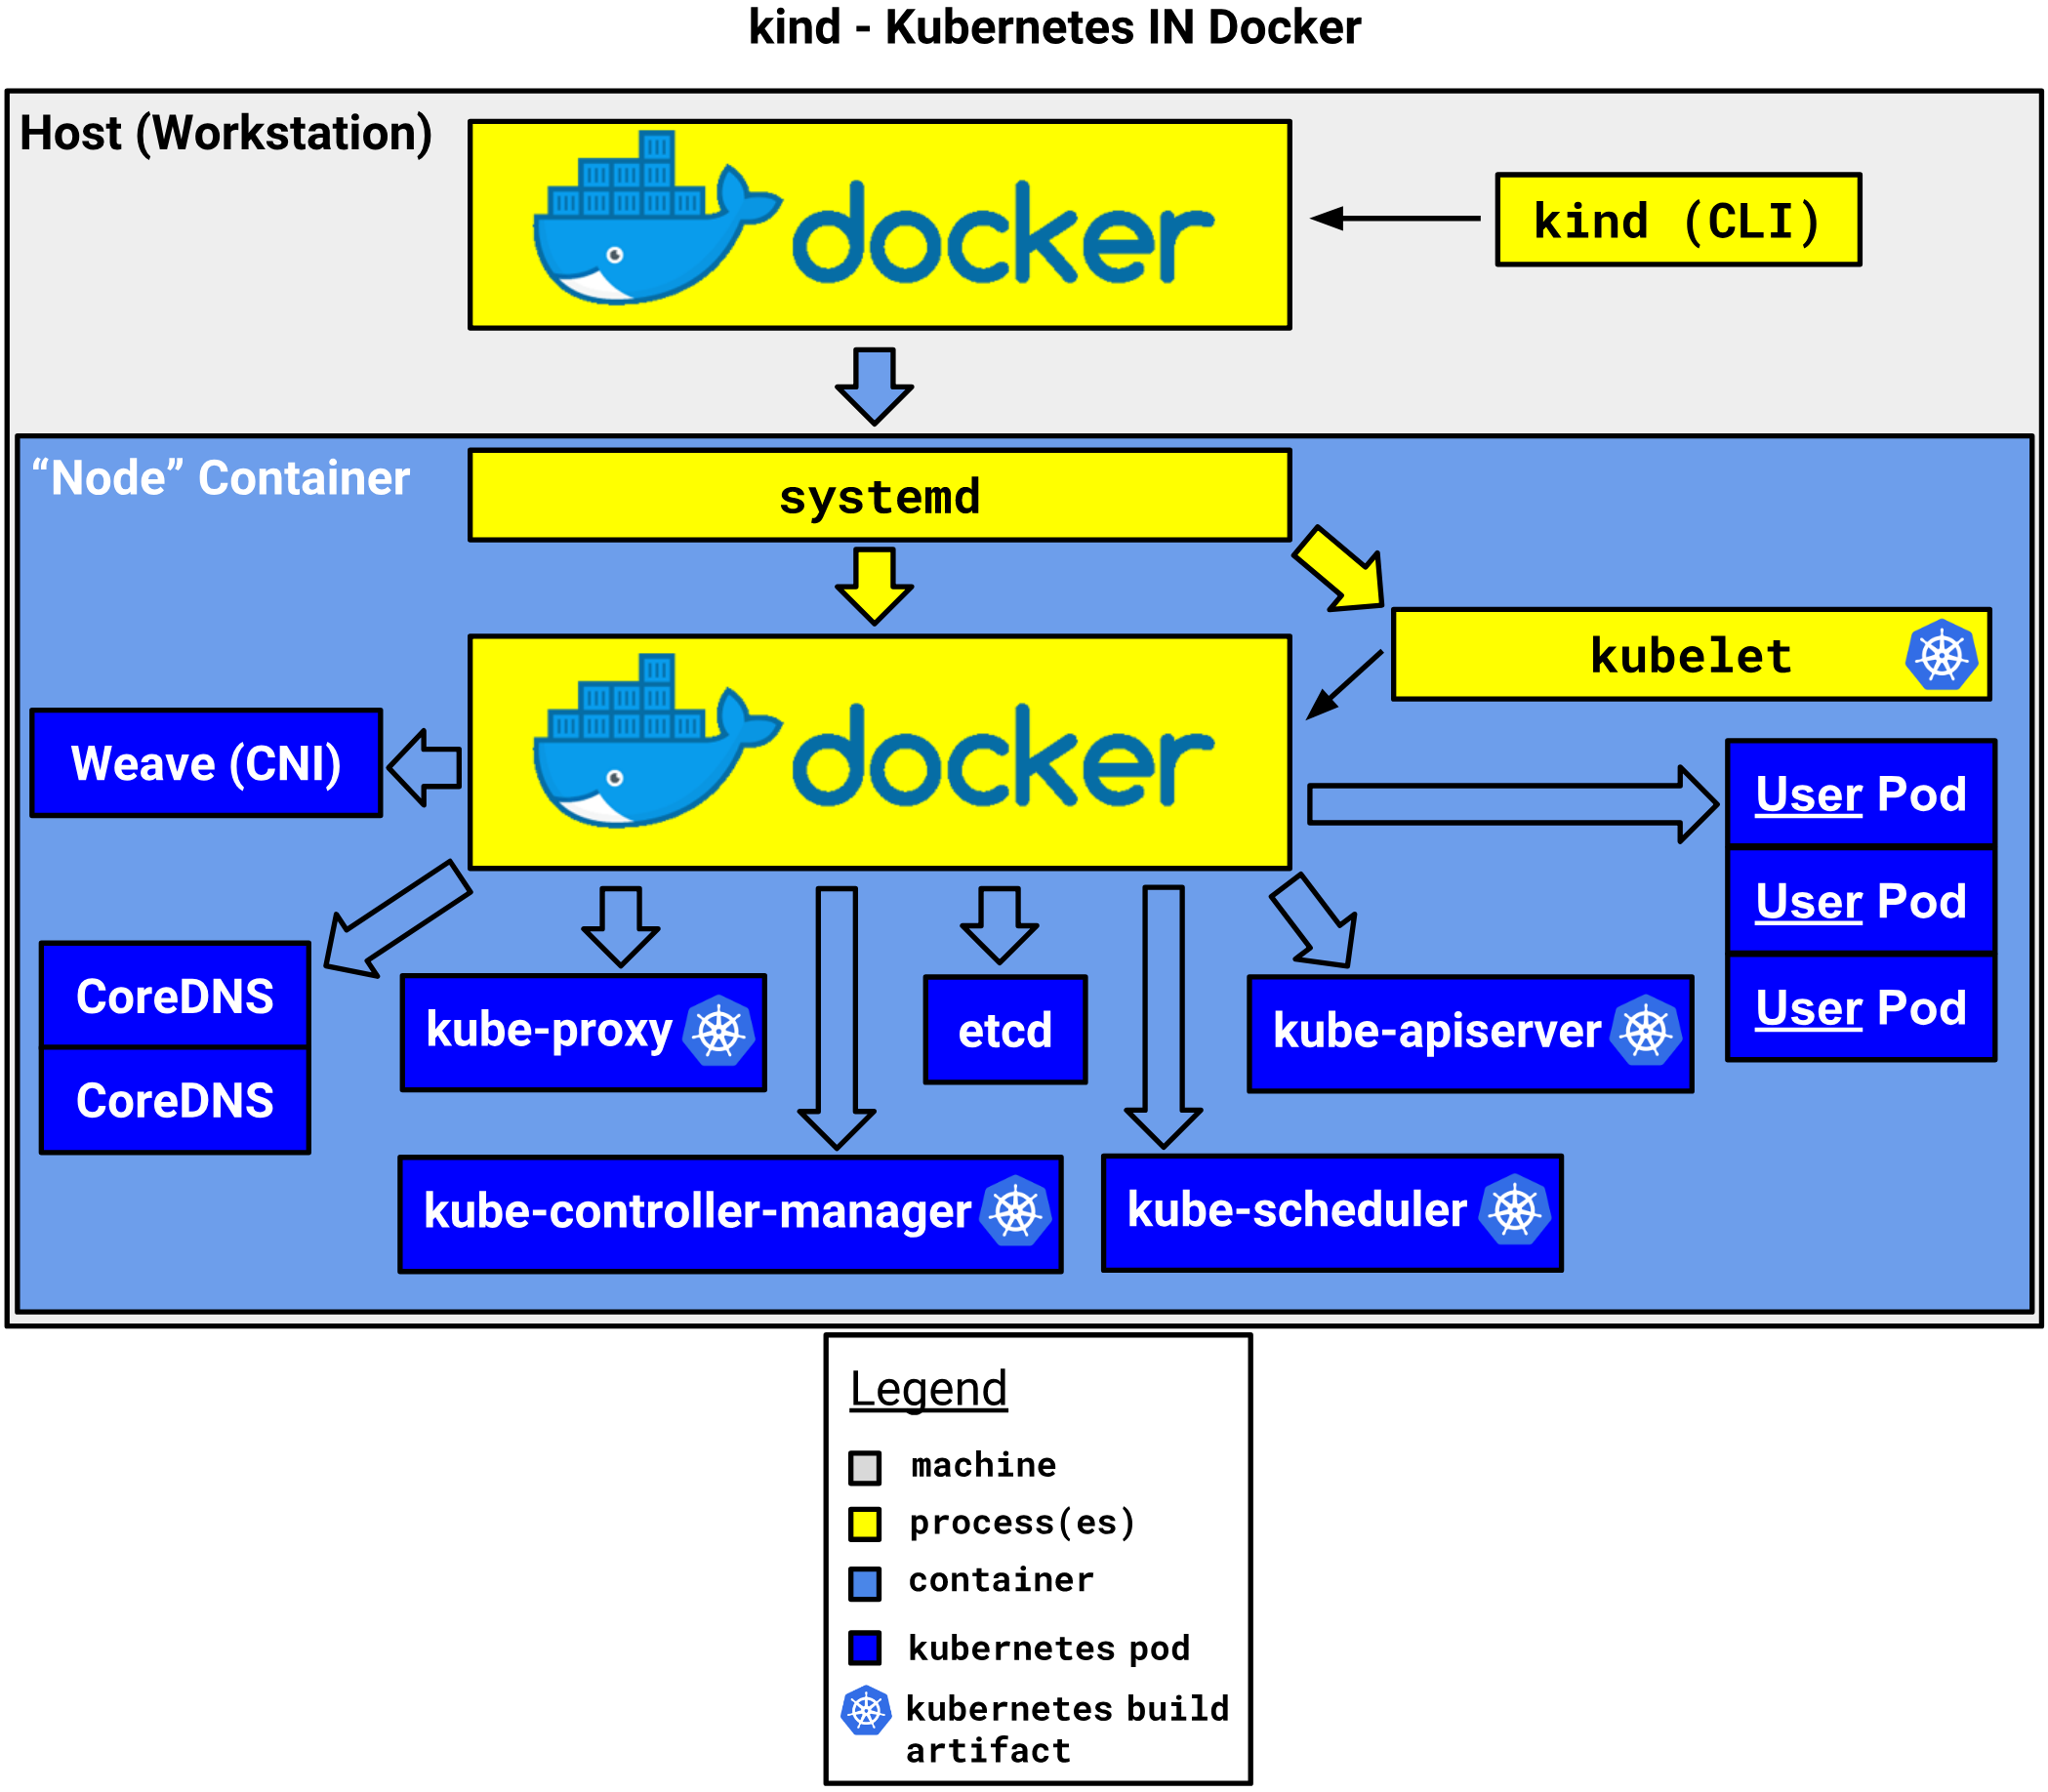
\includegraphics[width=0.85\textwidth]{figures/kubernetes/kind-overview-mod.png}
          \caption{KinD felépítése a gyakorlatban \cite{KinD}.}
           \label{kind-overview}
\end{figure}